\begin{center}
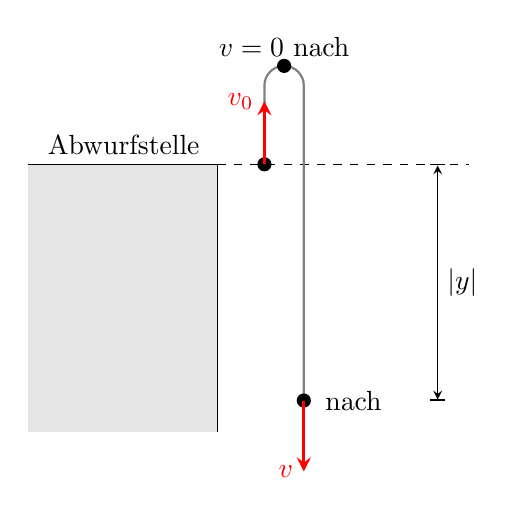
\begin{tikzpicture}[>=stealth]
 \fill[gray!20] (-3,0) rectangle (-0.6,-3.4);
 \draw (-3,0) -- (-0.6,0) -- (-0.6,-3.4);
 \draw[dashed] (-0.6,0) -- (2.6,0);
 \node[anchor=south east] at (-0.7,0) {Abwurfstelle};
 \draw[gray, thick] (0,0) -- (0,1) arc (180:0:0.25) -- (0.5,-3);
 \fill (0,0) circle (0.09);
 \draw[->, very thick, red] (0,0) -- (0,0.8) node[left] {$v_0$};
 \fill (0.25,1.25) circle (0.09) node[above] {$v = 0$ nach \tobO};
 \fill (0.5,-3) circle (0.09);
 \draw[->, very thick, red] (0.5,-3) -- (0.5,-3.9) node[left] {$v$};
 \node[anchor=west] at (0.65,-3) {nach \tgsO};
 \draw[|<->|] (2.2,0) -- (2.2,-3) node[midway, right] {$|y|$};
\end{tikzpicture}
\end{center}

Die Richtung nach oben ist positiv. Im höchsten Punkt ist die Geschwindigkeit null, also $0 = v_0 - g\,t_\mathrm{o}$ und
\begin{align}
 v_0 &= \voF = \gE\cdot\tob = \vo
\end{align}
Nach $t = \tgsO$ ist die Geschwindigkeit
\begin{align}
 v &= \vtF = \vo-\gE\cdot\tgs = \vt
\end{align}
Der Stein fliegt also mit $\result{\vabP{0}{2}}$ nach unten.

Da sich die Geschwindigkeit gleichmässig ändert, ist die mittlere Geschwindigkeit der Mittelwert aus Anfangs- und Endgeschwindigkeit:
\begin{align}
 \bar v &= \vmF = \frac{\vo+\left(\vt\right)}{2} = \vm
\end{align}
Die Lage relativ zur Abwurfstelle ist damit
\begin{align}
 y &= \yF = \left(\vm\right)\cdot\tgs = \y
\end{align}
Der Stein ist $\result{\yabP{0}{2}}$ unterhalb der Abwurfstelle.
